\chapter{Introduction to Calculus III: Parametric and Polar}

We begin by briefly thinking about the word \emph{dimension}.

\begin{exercise}{Dimension \Coffeecup} 
One intuitive notion of dimension comes from the idea of how you would assign units to measure it.  If an object has length, you would call it one-dimensional.  If an object has area, it is called two-dimensional.  If it has volume, it is called three-dimensional.  State the dimension of each of the following objects:

\begin{itemize}
\item $\lbrace x\in\mathbb{R} : x<2 \rbrace$
\item $\lbrace (x,y)\in\mathbb{R}^2 : x<2 \rbrace$
\item The closed interval $[2,3]$
\item The circle $\lbrace (x,y)\in\mathbb{R}^2 : x^2+y^2=1 \rbrace$
\item The disc $\lbrace (x,y)\in\mathbb{R}^2 : x^2+y^2\leq 1 \rbrace$
\end{itemize}
\end{exercise}

In Calculus III, you will redo all of the key concepts of Calculus I and II but in three (or more) dimensions.  Often the difficultly of higher-dimensional calculus is notational more than anything!  In three or more dimensions, it becomes messier to write down the same concepts.  To make this cleaner, we develop better languages for points and curves beyond our standard coordinate system.

\section{Parametric Curves}

Many of the objects we study, like circles or graphs of functions, are one-dimensional objects even though we usually view them as embedded in a two-dimensional plane.  Thus, we can represent both $x$ and $y$ (the two dimensions) in terms of the same parameter $t$.

\begin{definition}{Parametric Curve}
Let $x(t)$ and $y(t)$ be functions of $t$ and let $D \subset \mathbb{R}$.  The corresponding \emph{parametric curve} is the set of points $$\lbrace\left(x(t),y(t)\right): t\in D \rbrace. $$ \end{definition}

Typically, $D$ is an interval or union of intervals.  We can \parametric{graph} most curves by just selecting $t$ values from the domain $D$ and plotting the corresponding points.  

\begin{exercise}{A Warm-up Parametric Curve \Coffeecup \Coffeecup} 
Consider the \graphing{parametric curve} $$\lbrace\left(2t,3t+1\right): t\in [-1,3] \rbrace. $$
That is, $x(t)= 2t $, $y(t)=3t+1$, and $-1 \leq t \leq 3$.
\begin{itemize}
\item Use the above formulas for $x(t)$ and $y(t)$ and the following $t$-values selected from $D=[-1,3]$ to fill out the following table:

\begin{center}
\begin{tabular}{|c|c|c|c|c|c|} \hline
$t$ & -1 & 0 & 1 & 2 & 3 \\ \hline
$x(t)$ & & & & & \\
$y(t)$ & & & & & \\ \hline
\end{tabular}
\end{center}

\item Plot those five points on the axes below.  What type of shape does it appear to be?

\begin{center}
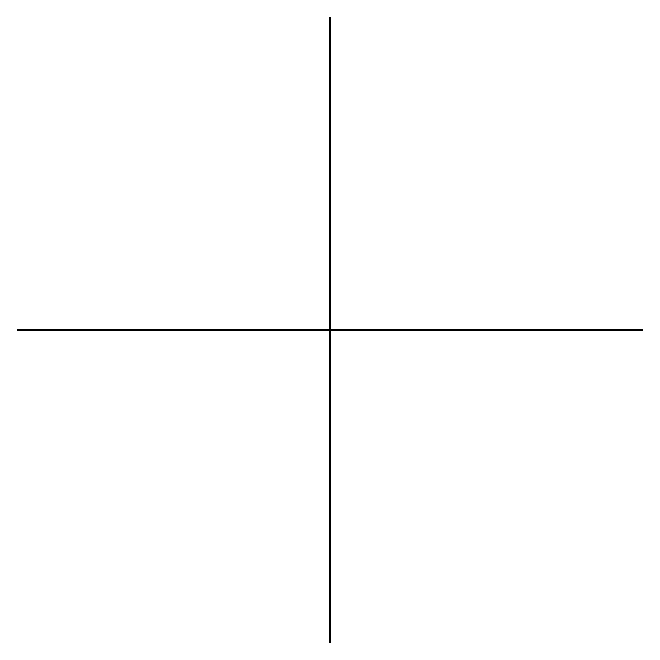
\includegraphics[scale=0.8]{quadall}
\end{center}

\item Solve the equation $ x= 2t$ for $t$.  Substitute this expression for $t$ into the equation $y=3t+1$.  What does this new equation tell you about the parametric curve?
\vspace*{1in}

\end{itemize} \AnswerKeyEntry{This parametric curve is the line $y=\frac{3}{2}x+1$.}
\end{exercise}

Here is an example of a parametric curve used in Trigonometry (though not called so at the time).

\begin{exercise}{The Unit Circle \Coffeecup \Coffeecup}
\begin{itemize}
\item Explain why the parametric curve $$C_1=\left\{\left(\cos(t),\sin(t)\right): t\in [0,2\pi] \right\}.$$ is the familiar unit circle from trigonometry.
\vspace*{1in}
\item Consider the curve $$C_2=\left\{\left(\sin(t),\cos(t)\right): t\in [0,2\pi] \right\}.$$ How are the curves $C_1$ and $C_2$ similar?  How are they different?
\vspace*{1in}
\end{itemize} \AnswerKeyEntry{The two curves are the same points in the plane.  Both start at the point (1,0) at time $t=0$, but $C_1$ then proceeds counter-clockwise while $C_2$ proceeds clockwise.}
\end{exercise}

\section{Derivatives of \tangentline{Parametric Curves}: Slopes of Tangent Lines}

To compute the derivative of a parametric curve, we recall that the slope of a line is the change in $y$-coordinate divided by the change in $x$-coordinate.  In the context of parametric curves, these can be computed as rates of change with respect to the parameter $t$.

\begin{definition}{Parametric Derivatives}
Let $\left(x(t),y(t)\right)$ be a \deriv{parametric} curve.  Then the slope of the tangent line can be computed as $$\frac{dy}{dx}=\frac{\frac{dy}{dt}}{\frac{dx}{dt}}.$$ 

	\begin{center}
		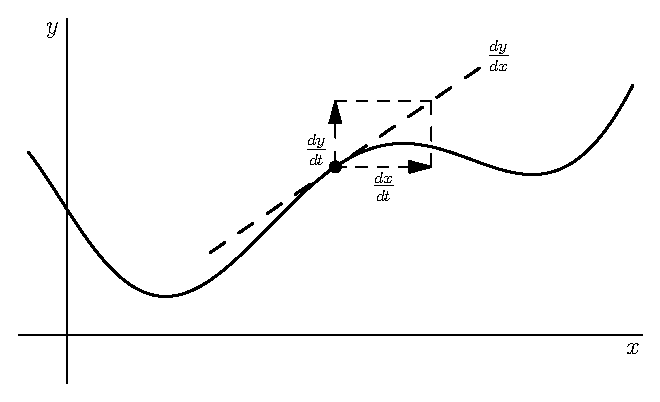
\includegraphics[width=270pt]{ChapterCalcIII/Figures/paraslope.eps}
	\end{center}

\end{definition}

Notice that the above formula is just a slightly rearranged version of the chain rule.  In particular, if we consider a portion of the graph of $\left(x(t),y(t)\right)$ that passes the Vertical Line Test, then we can consider $y$ as a function of $x$, which $x$ in turn is a function of $t$.  So if we wanted to ask how $y$ changes with respect to $t$, we would have to take the rate of change of $y$ with respect to $x$ and multiply it by the rate of change of $x$ with respect to $t$ (by the chain rule).  Expressing this Chain Rule in symbols instead of words, we have

$$\frac{ dy}{dt }=\frac{dy}{dx }\cdot \frac{dx}{dt }. $$

\begin{exercise}{Understanding the Definition \Coffeecup}
How would you get from the chain rule application shown above to our definition of parametric derivatives?
\vspace*{.5in}
\end{exercise}

\begin{example}{Parametric Derivatives on a Parabola}
Consider the \parabola{parametric curve} given by  $$\left\{\left(t^2,t\right): t\in [0,\infty) \right\}.$$ 

To find the slope of a tangent line to this \conics{parabola}, we can use the parametric \parametric{derivative} formula as follows:

\begin{align*}
\frac{dy}{dx}&=\frac{\frac{dy}{dt}}{\frac{dx}{dt}} \\
 &=\frac{\frac{d}{dt}\left( t\right)}{\frac{d}{dt}\left( t^2\right)} \\
 &=\frac{1}{2t}.\\
\end{align*}

Alternately, we could convert the curve to a cartesian equation and differentiate with respect to $y$.  Proceeding, we notice this curve is contained in the graph of $y=\sqrt{x}$, since the formulas $x=t^2$ and $y=t$ satisfy that relationship.  Thus, we can differentiate $y$ with the power rule.

\begin{align*}
\frac{dy}{dx}&=\left( \sqrt{x}\right)' \\
&=\frac{1}{2\sqrt{x}}
\end{align*}
\end{example}

\begin{exercise}{Equivalence of the Results \Coffeecup \Coffeecup}
In the above example, we have two distinct expressions for $\frac{dy}{dx}$.  Explain why they are in fact equivalent. \vspace*{1in} 
\end{exercise}

\begin{exercise}{The Tangent Line to an Ellipse \Coffeecup \Coffeecup}

\begin{itemize}
\item Plot the \ellipse{parametric} curve given by $$\left\{\left(2\cos(t),\sin(t)\right): t\in [0,2\pi] \right\}.$$ 

\begin{center}
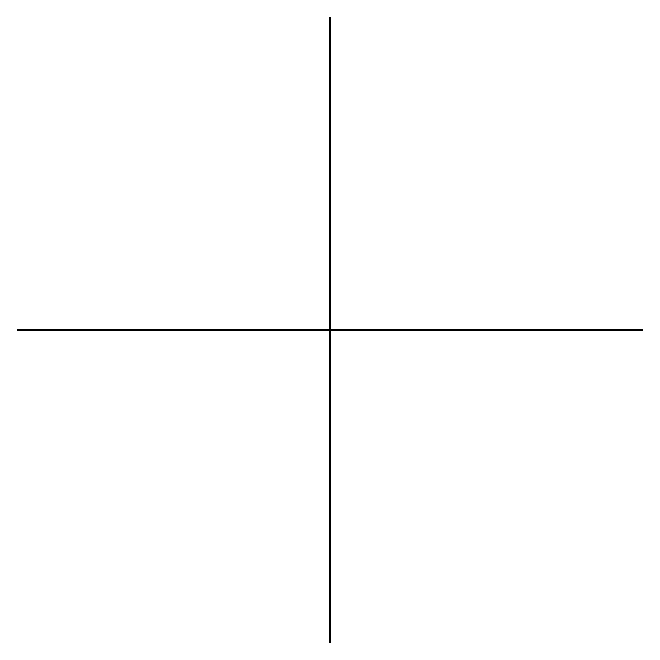
\includegraphics[scale=0.8]{quadall}
\end{center}

\item Find the point on the graph located at $t=\pi/4$, and find the slope of the tangent line at that point using the parametric derivative formula.  Sketch the tangent line on your graph above.

\vspace*{1in}

\item Verify the above curve is in fact the \conics{ellipse} given by $\frac{x^2}{4}+y^2=1$.

\vspace*{1in}

\item Use implicit differentiation on the equation $\frac{x^2}{4}+y^2=1$ to find $\frac{dy}{dx}$ at that same point and verify your answers match!
\vspace*{1in}
\end{itemize}
\end{exercise}

\begin{exercise}{Finding a Parameterization \Coffeecup \Coffeecup \Coffeecup}
 Find a parameterization of the path that consists of two full clockwise laps around the ellipse given by $$ \frac{(x-3)^2}{4}+(y-3)^2=1$$
starting from the point (3,2).
\vspace*{1in}
\end{exercise}

\begin{exercise}{A Hyperbola \Coffeecup \Coffeecup}
Consider the parametric curve given by the following: \begin{align*} x(t)&=e^t-e^{-t}, \\
y(t)&=e^t+e^{-t}, \\ t&\in [0,\infty).
\end{align*}
\begin{itemize}
\item Show that the above curve is contained in the hyperbola $y^2-x^2=4$.
\vspace*{2in}
\item Graph the parametric curve.
\begin{center}
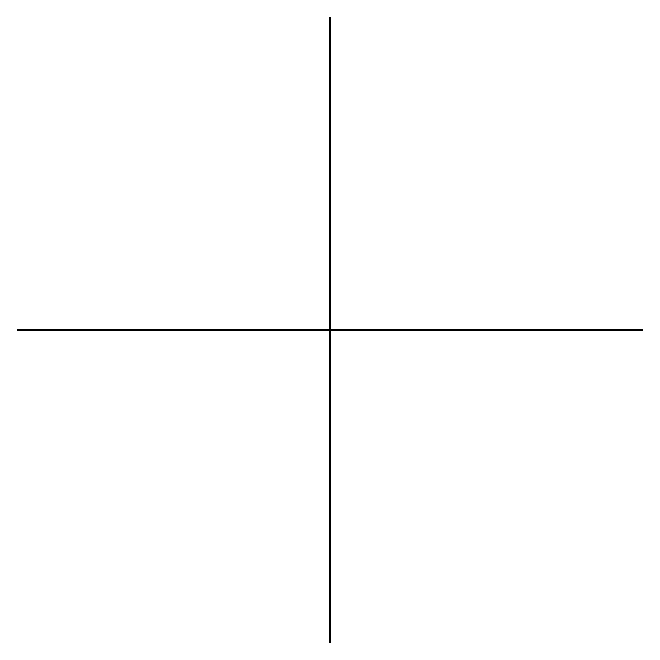
\includegraphics[scale=0.8]{quadall}
\end{center}
\item Find $dy/dx$ using the parametric formula for derivatives.  Take the limit as $t$ approaches infinity and interpret on your graph.
\vspace*{2in}
\end{itemize}
\end{exercise}

\section{Integrals of Parametric Curves: \parametric{Arc Length}}

The \arclength{length of a parametric curve} is given by the following formula.

\begin{theorem}{Parametric Arc Length }
Let a parametric curve $C$ be given by $\left(x(t),y(t) \right)$ for $a\leq t \leq b$.  Then the \integ{arc length} is computed via $$\int_{t=a}^{t=b}\sqrt{\left(\frac{dx}{dt}\right)^2+\left(\frac{dy}{dt}\right)^2} \dif t.$$
\end{theorem}

	\begin{center}
		\includegraphics[width=350pt]{ChapterCalcIII/Figures/paraarclength.eps}
	\end{center}

The construction here is nearly identical to the construction of the arc length of the graph of a function in Section \ref{ArcLength}.  We select points corresponding to $t$-values along the curve, compute the sum of the lengths of the line segments connecting them, and take the limit as the number of line segments goes to infinity.

\begin{exercise}{Fill in the Blanks!  Derivation of the Arc Length Formula \Coffeecup \Coffeecup}

Let $t_0,t_1,t_2,\ldots,t_n$ be equally spaced points in the interval $[a,b]$.  That is, $t_0=a$, $t_n=b$, and for each $i\in\lbrace 0,1,2,\ldots , n-1 \rbrace$, $\Delta t = \underline{\hspace{1.5in}}$.

With this setup, if we want the length of a line segment connecting points $\left(x\left(t_{i+1}\right),y\left(t_{i+1}\right)\right)$ and $\left(x\left(t_{i}\right),y\left(t_{i}\right)\right)$, we would use the Pythagorean Theorem to obtain 
$$\sqrt{ \binom{\hspace{1.5in}}{\hspace{1.5in}} } $$ as the length.

\begin{align*}
L&=\lim_{n\rightarrow \infty}\sum_{i=0}^{n-1} \sqrt{\hspace{1.5in}} \\
&=\lim_{n\rightarrow \infty}\sum_{i=0}^{n-1} \sqrt{\hspace{1.5in}} \sqrt{\left(\Delta t\right)^2} \\
&=\lim_{n\rightarrow \infty}\sum_{i=0}^{n-1} \sqrt{\hspace{1.5in} } \Delta t \\
&=\int_{t=a}^{t=b} \sqrt{\left(\frac{dx}{dt}\right)^2+\left(\frac{dy}{dt}\right)^2 } \dif t
\end{align*}
\end{exercise}

As usual, when first trying out a new tool, it is best to use it in a case where you already know the answer.

\begin{exercise}{Checking the Circumference of a Circle \Coffeecup \Coffeecup}  Consider the parametrization
$$ x(t)=r\cos(t)$$
$$ y(t)=r\sin(t)$$
for $t\in [0,2\pi]$.
\begin{itemize}
\item Explain why this is a parameterization of a circle of radius $r$.  
\vspace*{1in}
\item Use the parametric arc length formula to compute the length of the curve.  Compare it to your known formula for the \circles{circumference} of a circle.  Does the answer make sense?
\vspace*{2in}
\end{itemize}
\end{exercise}

\begin{exercise}{A Familiar Conic in Disguise \Coffeecup \Coffeecup \Coffeecup}

 Consider the parametrization 

\begin{align*}
 x(t)&=\sqrt{|t|} \\
 y(t)&=3t-1
\end{align*}

for $t\in [-2,2]$.
\begin{itemize}
\item Convert this to a cartesian equation.  What kind of shape is it?  

\vspace*{1in}

\item Sketch the curve.  Indicate any vertical or horizontal tangent lines and where they occur.

\begin{center}
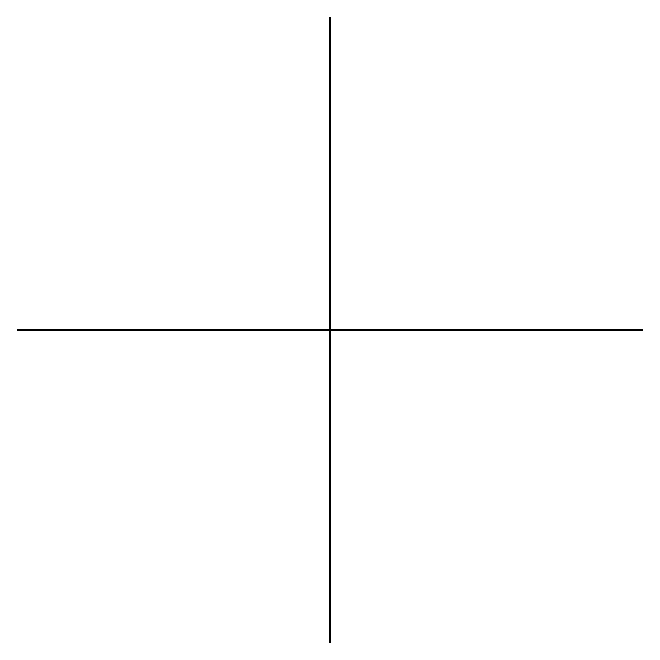
\includegraphics[scale=0.8]{quadall}
\end{center}

\item Use the parametric arc length formula to compute the length of the curve.  Does the answer make sense?
\vspace*{3in}
\end{itemize}
\AnswerKeyEntry{The arc length is $$\frac{6\sqrt{146}+\ln\left(\sqrt{73}+6\sqrt{2}\right)}{6}\approx 12.55.$$  Also, to handle the absolute value, just find the arc length on the interval [0,2] where you can ignore the absolute value and then apply symmetry.}
\end{exercise}

Ok, time to finally play with a curve that is not just a conic.

\begin{exercise}{Analyzing a Stranger Curve \Coffeecup \Coffeecup \Coffeecup}

\begin{itemize}
\item Sketch the graph of the following parametric curve $C$: $$ C=\left\{ \left( e^t\cos(t),e^t\sin(t)\right): 0\leq t\leq 2\pi\right\}.$$

Include labels of points on the graph at $t=0,\frac{\pi}{2},\pi, \frac{3\pi}{2}, 2\pi$.

\begin{center}
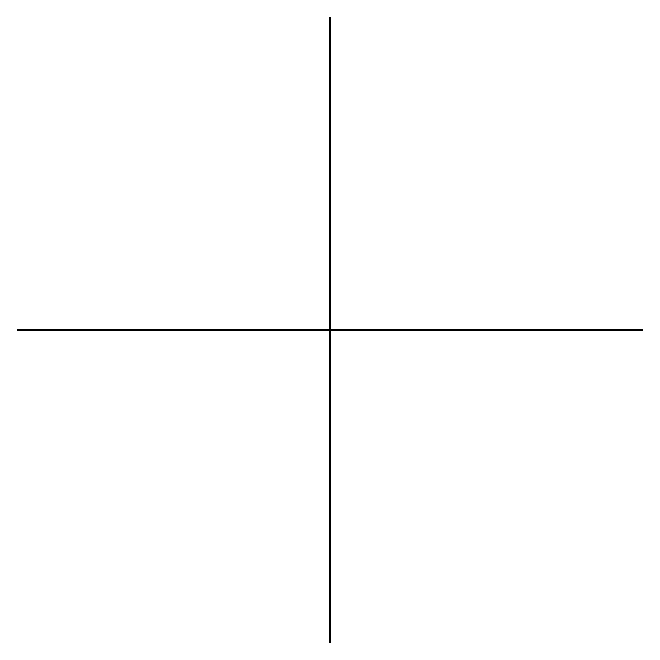
\includegraphics[scale=0.8]{quadall}
\end{center}

\item Where does the above graph have vertical tangent lines?  Where does the above graph have horizontal tangent lines?  Mark them on your graph.

\vspace*{1in}

\item What is the length of $C$?

\vspace*{1in}

\end{itemize}
\AnswerKeyEntry{The arc length is $\sqrt{2}\left(e^{2\pi}-1\right)$.}
\end{exercise}

\section{Hyperbolic \hyperbolic{Sine} and \hyperbolic{Cosine}}

You may have seen in a previous course (or if not, then here they are!) the definitions of the \emph{hyperbolic sine} and \emph{hyperbolic cosine} functions.  They are typically defined as follows:

\begin{itemize}
\item $\cosh(t)=\frac{e^t+e^{-t}}{2}$
\item $\sinh(t)=\frac{e^t-e^{-t}}{2}$
\end{itemize}

This of course prompts the question: ``why do these $e$ things get called sine or cosine?''  We answer this question below.

\begin{exercise}{Power Series for Hyperbolic Sine and Cosine \Coffeecup \Coffeecup}
\begin{itemize}
\item Find a power series for $\cosh$ by using what we know about the series for the exponential function.  How does the resulting series relate to cosine?

\vspace*{2in}

\item Find a power series for $\sinh$ by using what we know about the series for the exponential function.  How does the resulting series relate to sine?
\vspace*{2in}
\end{itemize}
\end{exercise}

And of course there are more questions prompted here: ``Why do these $e$ things get called \cosine{hyperbolic}?  What do these \conics{hyperbolic functions} have to do with hyperbolas?''

\begin{exercise}{Parametric Curve Generated by Hyperbolic Sine and Cosine \Coffeecup \Coffeecup \Coffeecup} Consider the parametric curve $$\left\{ (\cosh(t),\sinh(t)): t\in \mathbb{R} \right\}.$$ 
\begin{itemize}
\item Verify this \hyperbola{parametric curve} satisfies the cartesian equation for a hyperbola given by $$x^2-y^2=1 $$ by plugging the exponential definitions for our \hyperbola{hyperbolic trig functions} in for $x$ and $y$.
\vspace*{2in}
\item Again, verify this parametric curve satisfies the cartesian equation for the same hyperbola given by $$x^2-y^2=1 $$
by plugging the power series formulas for our hyperbolic trig functions in for $x$ and $y$. \vspace*{3in}
\end{itemize}
\end{exercise}